% parallel_workflow.tex - 并行多模块实验流程图模板 (Parallel Experimental Workflow)
% 编译方式: pdflatex parallel_workflow.tex 或 xelatex parallel_workflow.tex
\documentclass[tikz,border=10pt]{standalone}
\usepackage{xcolor}
\usepackage{tikz}
\usetikzlibrary{arrows.meta, positioning, calc, shapes.geometric, backgrounds, fit}

\definecolor{natureblue}{HTML}{4E79A7}
\definecolor{natureorange}{HTML}{F28E2B}
\definecolor{naturered}{HTML}{E15759}
\definecolor{naturecyan}{HTML}{76B7B2}
\definecolor{naturegreen}{HTML}{59A14F}
\definecolor{darktext}{HTML}{262626}
\definecolor{subtext}{HTML}{6C757D}
\definecolor{lightbg}{HTML}{F8F9FA}
\definecolor{boxborder}{HTML}{CBD5E1}

\begin{document}
\sffamily
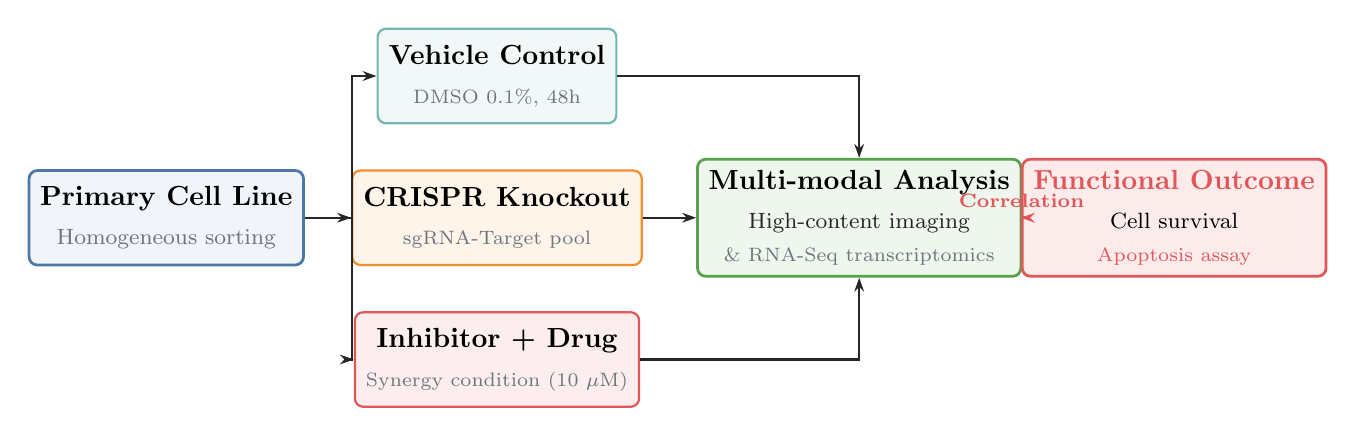
\begin{tikzpicture}[
    node distance=1.2cm and 1.8cm,
    block/.style={
        rectangle,
        rounded corners=3pt,
        draw=boxborder,
        fill=lightbg,
        line width=0.8pt,
        minimum width=2.8cm,
        minimum height=1.2cm,
        inner sep=4pt,
        align=center
    },
    hub/.style={
        block,
        draw=natureblue,
        fill=natureblue!8,
        line width=1.0pt,
        minimum width=3.2cm
    },
    armA/.style={
        block,
        draw=naturecyan,
        fill=naturecyan!10
    },
    armB/.style={
        block,
        draw=natureorange,
        fill=natureorange!10
    },
    armC/.style={
        block,
        draw=naturered,
        fill=naturered!10
    },
    converge/.style={
        block,
        draw=naturegreen,
        fill=naturegreen!10,
        minimum width=3.4cm,
        line width=1.0pt
    },
    arrow/.style={
        -{Stealth[length=5pt,width=3.5pt]},
        line width=0.8pt,
        color=darktext
    }
]

    % --- 起始统一处理节点 ---
    \node[hub] (origin) at (0, 0) {
        {\bfseries Primary Cell Line}\\[2pt]
        {\footnotesize\color{subtext} Homogeneous sorting}
    };

    % --- 并行三实验分支 (Parallel Arms) ---
    \node[armA] (arm1) at (4.2, 1.8) {
        {\bfseries Vehicle Control}\\[2pt]
        {\scriptsize\color{subtext} DMSO 0.1\%, 48h}
    };

    \node[armB] (arm2) at (4.2, 0.0) {
        {\bfseries CRISPR Knockout}\\[2pt]
        {\scriptsize\color{subtext} sgRNA-Target pool}
    };

    \node[armC] (arm3) at (4.2, -1.8) {
        {\bfseries Inhibitor + Drug}\\[2pt]
        {\scriptsize\color{subtext} Synergy condition ($10\ \mu\mathrm{M}$)}
    };

    % --- 汇聚综合分析节点 ---
    \node[converge] (analysis) at (8.8, 0) {
        {\bfseries Multi-modal Analysis}\\[2pt]
        {\footnotesize\color{darktext} High-content imaging}\\
        {\scriptsize\color{subtext} \& RNA-Seq transcriptomics}
    };

    % --- 终极表型输出 ---
    \node[block, draw=naturered, fill=naturered!12, line width=1.0pt, minimum width=2.8cm] (outcome) at (12.8, 0) {
        {\bfseries\color{naturered} Functional Outcome}\\[2pt]
        {\footnotesize Cell survival}\\
        {\scriptsize\color{naturered} Apoptosis assay}
    };

    % --- 分流连接箭头 (Bifurcation) ---
    \draw[arrow] (origin.east) -- ++(0.6,0) |- (arm1.west);
    \draw[arrow] (origin.east) -- (arm2.west);
    \draw[arrow] (origin.east) -- ++(0.6,0) |- (arm3.west);

    % --- 汇流连接箭头 (Convergence) ---
    \draw[arrow] (arm1.east) -- ++(0.6,0) -| (analysis.north);
    \draw[arrow] (arm2.east) -- (analysis.west);
    \draw[arrow] (arm3.east) -- ++(0.6,0) -| (analysis.south);

    % --- 终点连接 ---
    \draw[arrow, line width=1.0pt, color=naturered] (analysis.east) -- node[above, font=\scriptsize\bfseries\color{naturered}] {Correlation} (outcome.west);

\end{tikzpicture}
\end{document}
